\section{Introduction}

\begin{figure}[t]
\centering
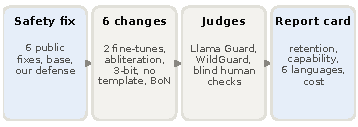
\includegraphics[width=\columnwidth]{figures/fig0_pipeline.pdf}
\caption{Aftermarket: every model goes through the same six post-release changes, two automatic judges checked
against blind human labels, and one report card.}
\label{fig:pipeline}
\end{figure}

An open-weight model is not a fixed artifact. Within days of a release, people fine-tune it on their own data,
quantize it to fit a phone, serve it from a raw completion endpoint without its chat template, or remove its refusals
on purpose with a single weight edit~\citep{arditi2024refusal}. A safety fix that holds only on the checkpoint its
authors published protects nobody who uses the model in any other form. Yet fixes are almost always evaluated on that
one checkpoint.

Each of these attacks is well documented on its own (\S\ref{sec:related}). What is missing is a common yardstick:
the same everyday post-release changes, applied with the same prompts, judges and statistics to every fix that
claims to make a model safer.

We build that yardstick, \emph{Aftermarket} (Fig.~\ref{fig:pipeline}), and apply it to every public safety fix for Tiny Aya Global
\citep{salamanca2026tinyaya} that we could load from a recent safety hackathon: six fixes spanning weight-space repair,
safety-aware fine-tuning, rank-one patches, and a prompt guard in the chat template. Our contributions:
\begin{enumerate}
\item \textbf{A shared post-release battery} of six changes, run on 12 models with identical seeds, prompts, two
  judges and paired statistics, plus capability, multilingual and serving-cost measurements\stagetwo{}
  (\S\ref{sec:setup}).
\item \textbf{A durability leaderboard} with one retention score, and the finding that release-time safety does
  not predict it (\S\ref{sec:survive}--\ref{sec:capability}).
\item \textbf{A judge audit} against blind hand labels in English and Yoruba: the pre-registered judge disagrees
  with a human far more than WildGuard on perturbed text, and judging Yoruba through back-translation overstates
  harm (\S\ref{sec:judges}, \S\ref{sec:multilingual}).
\item \textbf{A tested defense and a negative result}: hardening the layers that carry the refusal direction makes
  a model safer at release but \emph{less} durable, and no better than random layers (\S\ref{sec:defense}).
\end{enumerate}
Our headline has two parts. First, most public safety fixes do not survive ordinary post-release changes, and how
safe a model is at release says little about how well that safety holds; the attacks that undo them leave
capability nearly intact. Second, the automatic tools used to measure safety can mislead: against blind hand
labels, the pre-registered Llama Guard judge agrees with a human at only $\kappa=\V{kappa.lg.all}$ in English, and
judging Yoruba replies through back-translation overstates harm several-fold (the author, a native Yoruba speaker, confirms
\V{humjudge.flag.yes} of \V{humjudge.flag.n} flagged replies) while still missing some. A fix should be tested in the
forms people actually run, with judges checked against humans in every language reported.
